
\chapter{A szimuláció eredményei}

Kezdetben a szimuláció pontosságának megvizsgálása érdekében a már rendelkezésünkre álló bemeneti paraméterekre (melyeket Archetti is használt\cite{archetti2016cooperation}) elvégeztünk 100-100 szimulációt, minden egyes diffúziós távolságra 1-től 5-ig.

\begin{multicols}{2}
	A bemeneti paraméterek a következőek voltak:
	\begin{itemize}[noitemsep]
		\item populáció mérete: 1000
		\item defektálók: 5\%
		\item generációk száma: 15
		\item kooperálók költsége: 0.01
		\item osztódás: nincs
	\end{itemize}
	Az \eqref{eq:payoffGradient} és \eqref{eq:diffGradient} függvények paraméterei, melyeket az elkövetkezendő szimulációk során használtunk:
	\begin{itemize}[noitemsep]
		\item $s = 2$
		\item $k = 1$
		\item $d = \frac{1}{2}D$
		\item $z = 20$
	\end{itemize}	
\end{multicols}

Megállapítottuk, hogy ugyanarra az eredményre (Ábra \ref{fig:DistChange}) jutottunk mi is mint Archetti\cite{archetti2016cooperation}, igaz kisebb eltérések ugyan mutatkoztak. Míg mi minden esetben 100 szimulálást végeztünk, addig ő csak 10-et, így a kis eltéréseket ennek tulajdoníthatjuk.

\begin{figure}[h]
	\centering
	\begin{tabular}{cc}
		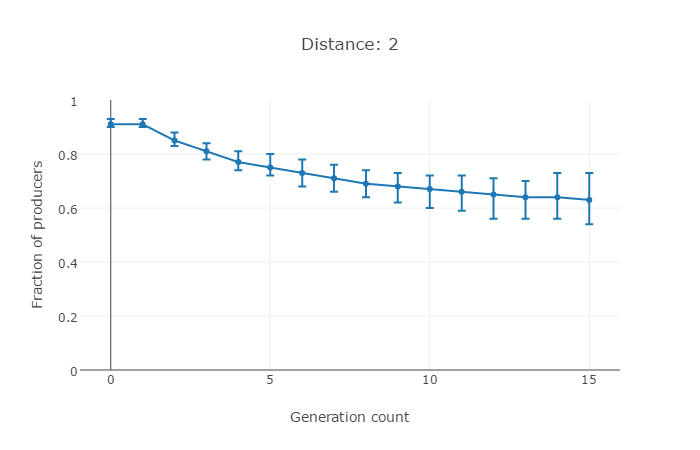
\includegraphics[width=0.47\linewidth]{images/dist2}
		&
		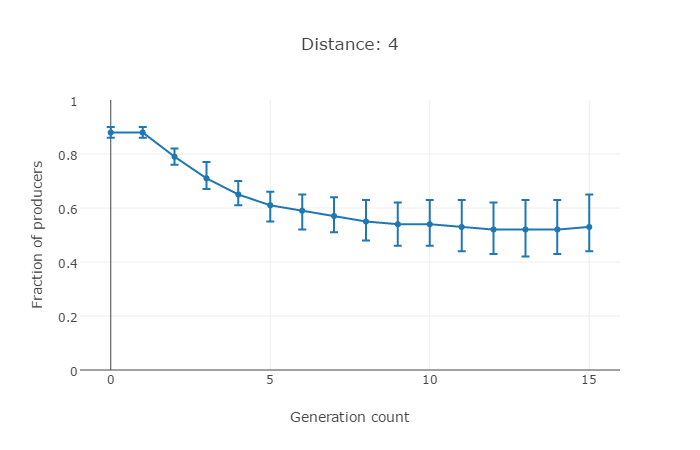
\includegraphics[width=0.47\linewidth]{images/dist4}
		\\
		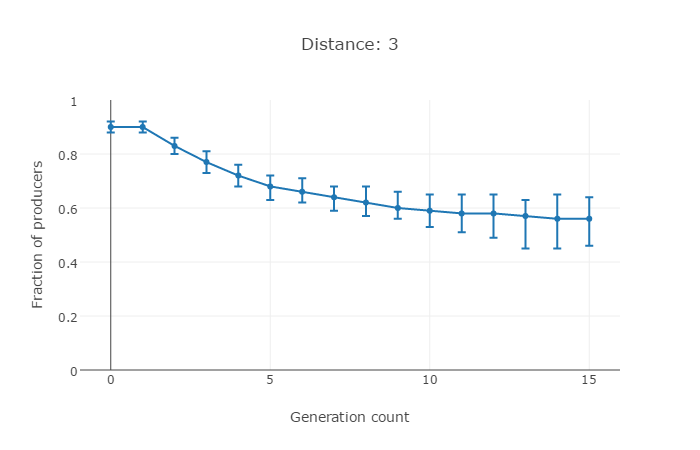
\includegraphics[width=0.47\linewidth]{images/dist3}
		&
		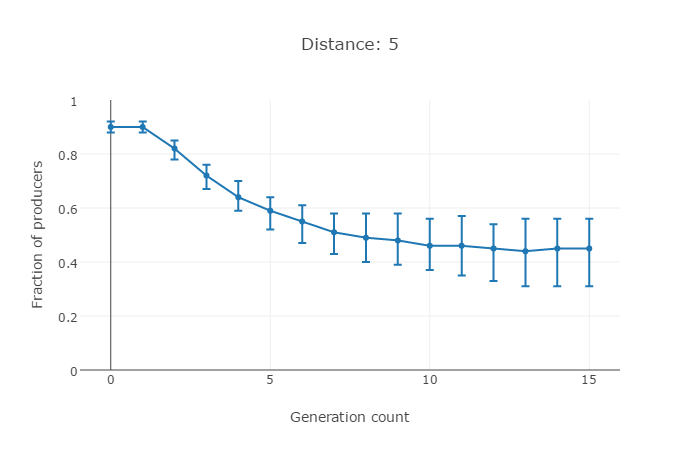
\includegraphics[width=0.47\linewidth]{images/dist5}
		\\
	\end{tabular}
	\caption{Szimulációs eredmények a fenti paraméterekre}
	\label{fig:DistChange}
\end{figure}

Ezzel projektünk első mérföldkövét leraktuk, így most már kísérletezhetünk különböző paraméterekkel, hogy megvizsgáljuk a populáció viselkedését. Egy pár esetet a következő fejezetekben tárgyalunk.

\section{A költség és nyereség hatása}

Mint ahogyan azt már láttuk, a kooperáló sejtek termelési költsége nagyban befolyásolja a játék végkimenetelét (Ábra \ref{fig:CoopCostChange}), ami nem nagy meglepetés, hisz minél többe kerül a termelés annál jobban megéri élősködni. Az esetek többségében a defektálás a legkifizetődőbb, de alacsony költségek mellett fenntartható egy bizonyos egyensúly is a két fél között, sőt, extrém körülmények (paraméterek) mellett az is elérhető, hogy a teljes populáció a kooperálás mellett döntsön.

\begin{figure}[h]
	\centering
	\begin{tabular}{ccc}
		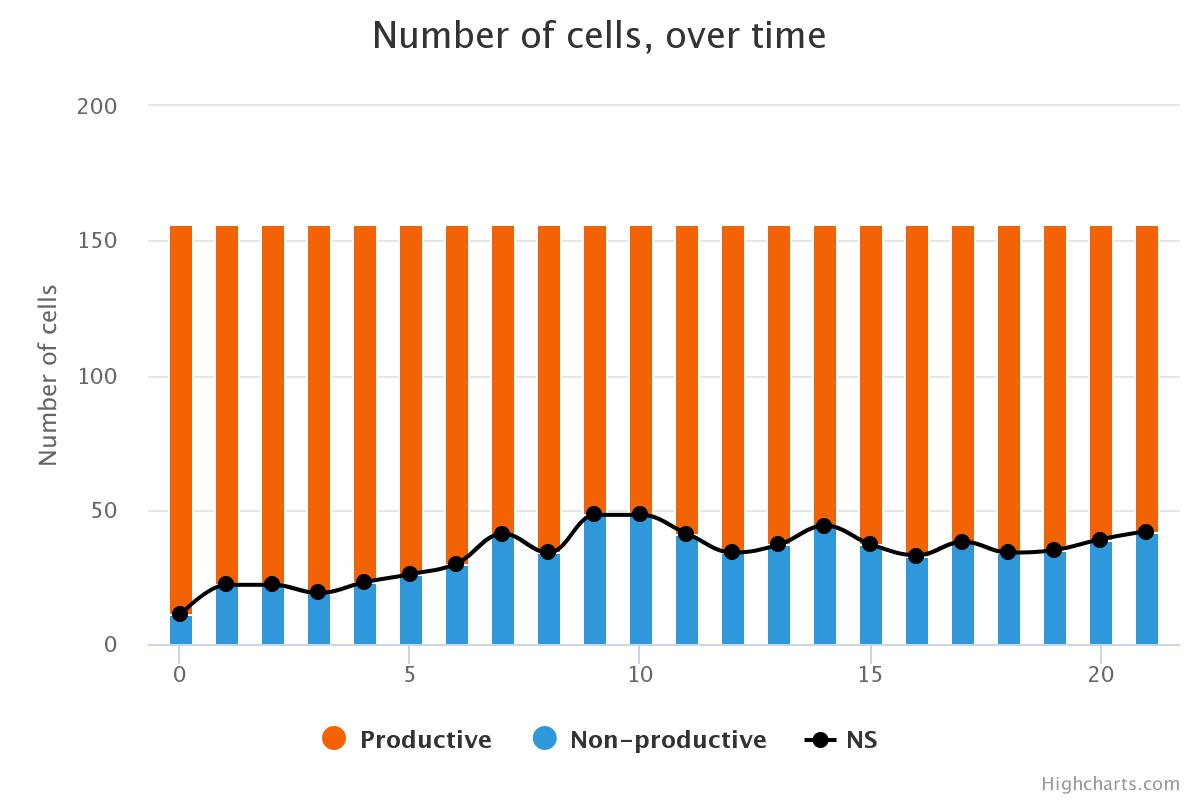
\includegraphics[width=0.32\linewidth]{images/chart001.jpeg}
		&
		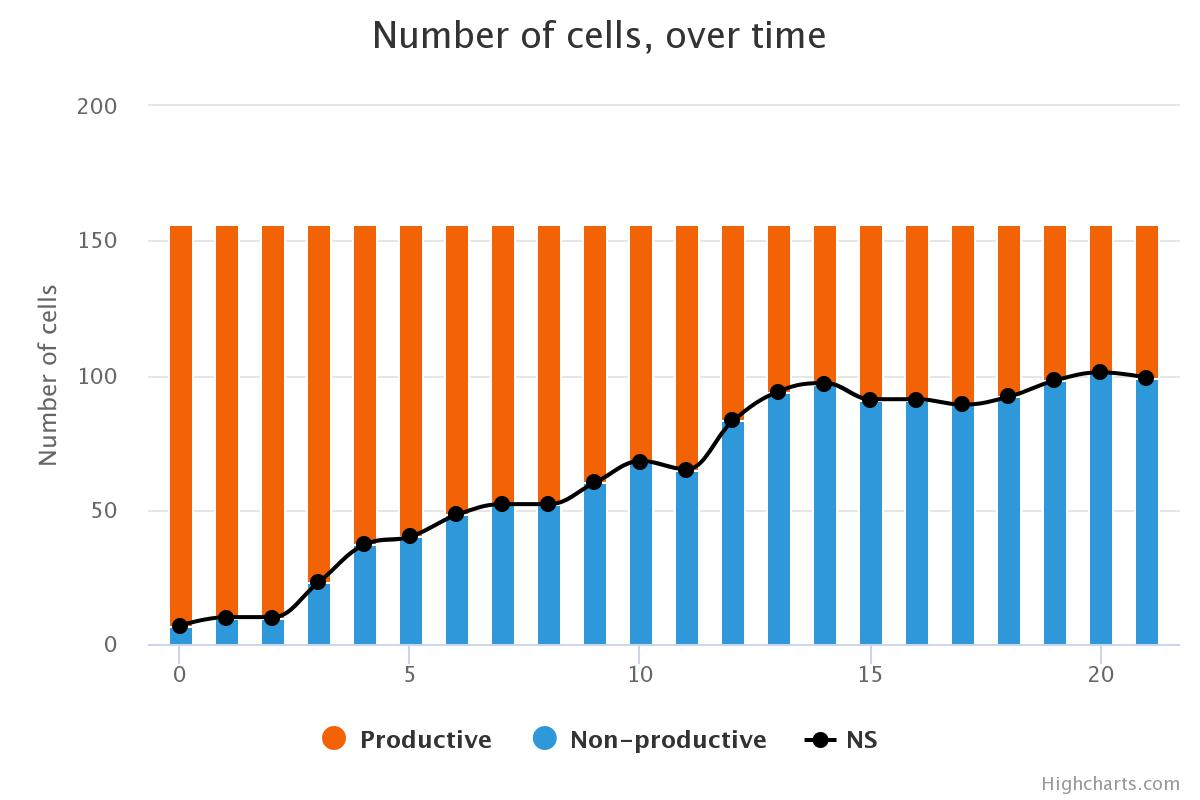
\includegraphics[width=0.32\linewidth]{images/chart01.jpeg}
		&
		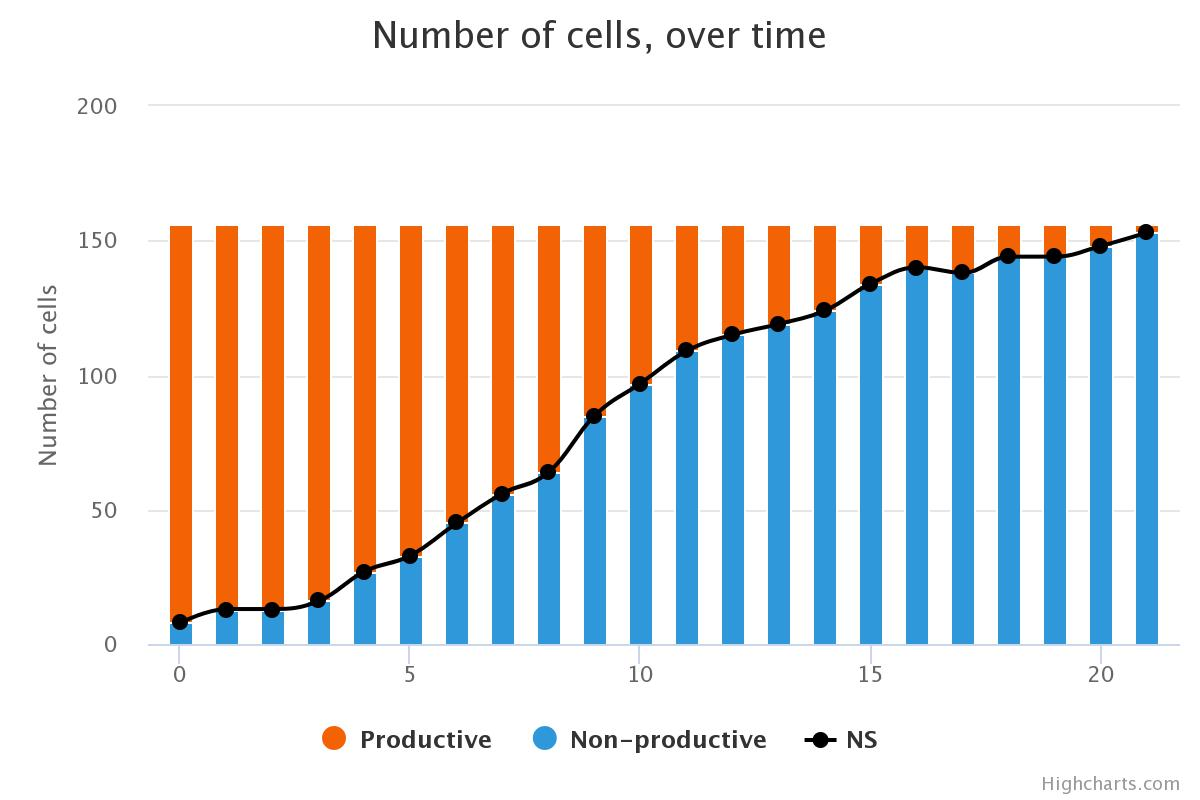
\includegraphics[width=0.32\linewidth]{images/chart08.jpeg}
	\end{tabular}
	\captionof{figure}{A játék végkimenetele mikor a költségek rendre 0.01, 0.1 és 0.8\label{fig:CoopCostChange}}
\end{figure}


\section{Diffúziós távolság hatása}

Egyik legkényesebb paraméterünk amelyet változtatni lehet, az a diffúziós távolság, amely növelésével valósághűbb adatokat kaphatunk. Sajnos nem állnak rendelkezésünkre erre vonatkozó adatok a biológiából, így csak egy pár, már más által is használt értékekre végeztünk kísérleteket (Ábra \ref{fig:DiffDist}).

\begin{figure}[h]
	\centering
	\begin{tabular}{cc}
		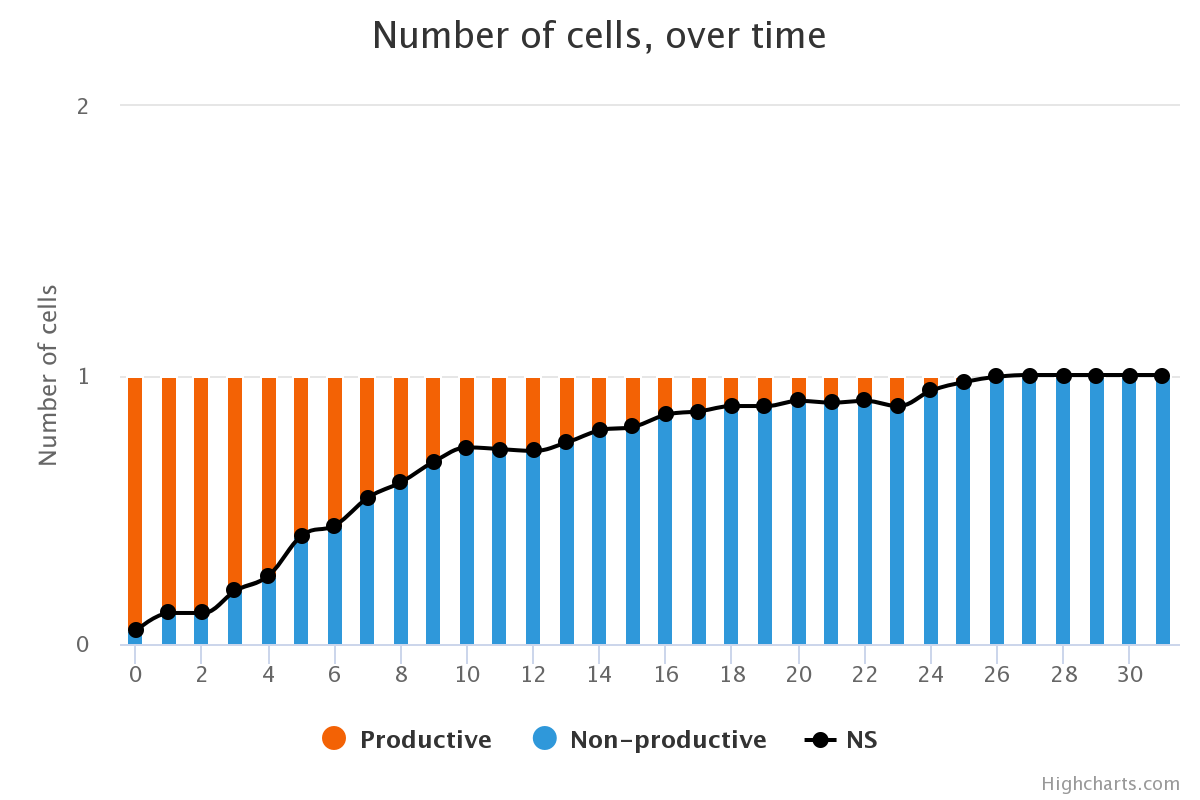
\includegraphics[width=0.47\linewidth]{images/diffdist2}
		&
		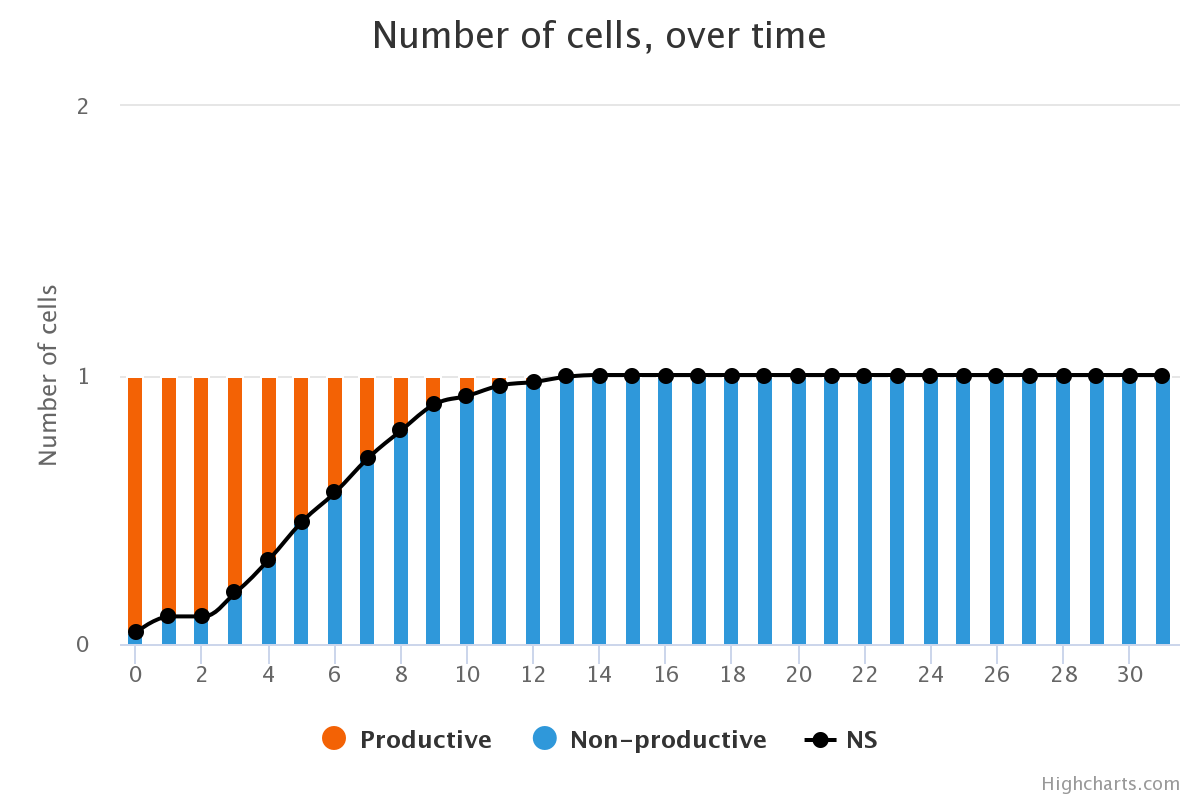
\includegraphics[width=0.47\linewidth]{images/diffdist5}
	\end{tabular}
	\caption{A játék végkimenetele két diffúziós távolságra. A paraméterek: 160 sejt, 5\% defektáló, 0.3 költség, távolság: 2 illetve 5}
	\label{fig:DiffDist}
\end{figure}

Megfigyelhető, hogy a távolság növekedésével a defektáló sejtek jóval könnyebben terjednek el, nem csak a közvetlen szomszédokat befolyásolják, hanem a tőlük távolabb elhelyezkedőeket is. Meg kell jegyeznünk, hogy ezt a paramétert a hasnyálmirigyrák esetén megállapították\cite{archetti2015heterogeneity}, valamint az is biztos, hogy az esetek túlnyomó részében ez az érték 5-10-től 30-60-ig terjedhet\cite{archetti2016cooperation}.
%További megvalósítandó feladataink közé tartozik egy olyan funkció mely révén ellenanyagot juttathatunk a daganatba, vagy egy terápiát alkalmazhatunk.
\section{Osztódásra képes populációk}

Eddigi szimulációink során a populáció mérete állandó volt, és egy adott modellt követett. Nézzük meg mi történik ha a sejtek osztódni is képesek nem csak stratégiát váltani (Ábra \ref{fig:Divide}). 

\noindent
\begin{minipage}{\linewidth}
	\centering
	\begin{multicols}{2}
		\begin{Figure}
			\centering
			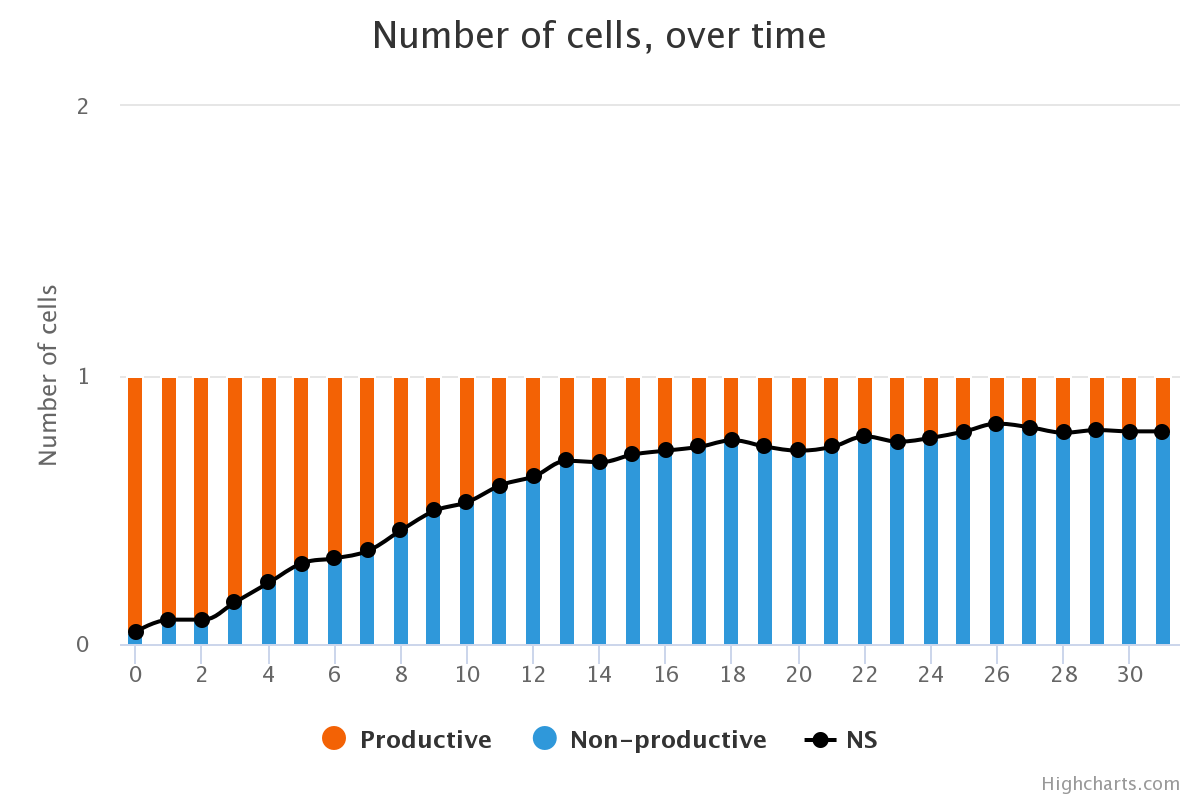
\includegraphics[width=\linewidth]{images/nemosztodik}
		\end{Figure}
		\begin{Figure}
			\centering
			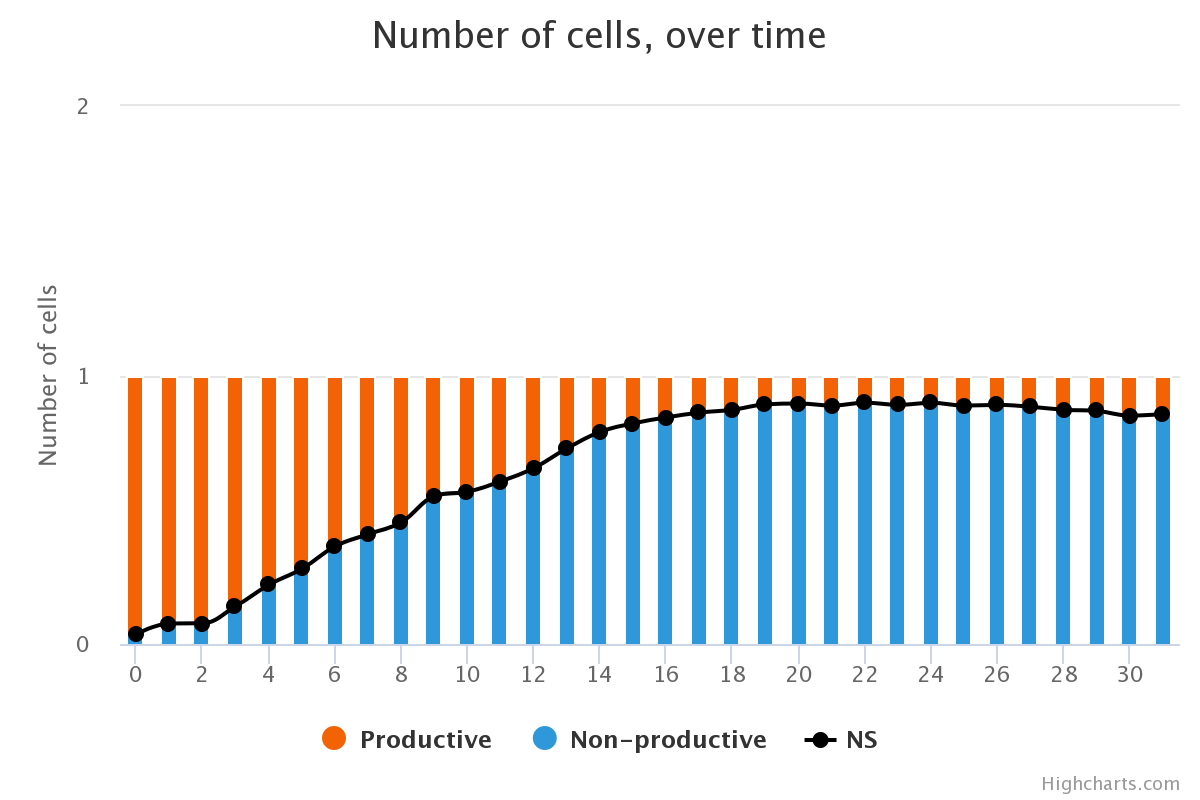
\includegraphics[width=\linewidth]{images/osztodik}
		\end{Figure}
	\end{multicols}
	\captionof{figure}{Az első esetben a sejtek nem osztódtak míg a másodikban igen \label{fig:Divide}}
\end{minipage}\\

Igaz, hogy a stratégia váltást fel lehet fogni úgy mint egy fajta osztódást, ahol az a sejt amelyik átveszi a stratégiát meghal és annak a sejtnek a másolata jön létre ugyanazon a területen akitől azt átveszi, de a valóságban a defektáló sejtek nem csak területileg terjednek el, hanem számosságban is túlnövik a kooperálókat.
Az osztódás során létrejött új sejtek képesek felgyorsítani a defektálók terjedését, de ezen területen még további kísérletek szükségesek, hogy pontosabb képet kapjunk arról, hogy ez mennyire befolyásolja a játék végkimenetelét.

Felhasználva a fenti paramétereket legeneráltunk egy újabb populációt mely már osztódásra képes (\ref{table:osztodik} táblázat), és ezen eredményeket összevetettük azon modellel ahol nem volt osztódás (\ref{table:nemOsztodik} táblázat). Látható, hogy a kooperálók aránya (CoopPerc) kisebb amikor a sejtek osztódnak, de a szórása is nő.

\begin{table}[htb]
	\caption{Osztódás nélküli modell}
	\label{table:nemOsztodik}
	\begin{tabular}{ | l | l | l | l | l | l | l | l | l | l | l | l | }
		\hline
		\multirow{3}{*}{D = 2}
		& Generáció & 1 & 2 & 3 & 4 & 5 & 6 & 7 & 8 & 9 & 10 \\ \cline{2-12}
		& CoopPerc & 0.91 & 0.91 & 0.85 & 0.81 & 0.77 & 0.75 & 0.73 & 0.71 & 0.69 & 0.68 \\ \cline{2-12}
		& stdev & 0.01 & 0.01 & 0.02 & 0.03 & 0.03 & 0.03 & 0.05 & 0.05 & 0.05 & 0.06 \\ \hline
		\multirow{3}{*}{D = 3}
		& Generáció & 1 & 2 & 3 & 4 & 5 & 6 & 7 & 8 & 9 & 10 \\ \cline{2-12}
		& CoopPerc & 0.9 & 0.9 & 0.83 & 0.77 & 0.72 & 0.68 & 0.66 & 0.64 & 0.62 & 0.6 \\ \cline{2-12}
		& stdev & 0.02 & 0.02 & 0.03 & 0.04 & 0.04 & 0.05 & 0.04 & 0.05 & 0.05 & 0.04 \\ \hline
	\end{tabular}
\end{table}

\begin{table}[htb]
	\caption{Osztódást használó modell}
	\label{table:osztodik}
	\begin{tabular}{ | l | l | l | l | l | l | l | l | l | l | l | l | }
		\hline
		\multirow{3}{*}{D = 2}
		& Generáció & 1 & 2 & 3 & 4 & 5 & 6 & 7 & 8 & 9 & 10 \\ \cline{2-12}
		& CoopPerc & 0.87 & 0.87 & 0.79 & 0.74 & 0.7 & 0.67 & 0.64 & 0.61 & 0.59 & 0.57 \\ \cline{2-12}
		& stdev & 0.02 & 0.02 & 0.03 & 0.04 & 0.05 & 0.06 & 0.07 & 0.05 & 0.07 & 0.07 \\ \hline
		\multirow{3}{*}{D = 3}
		& Generáció & 1 & 2 & 3 & 4 & 5 & 6 & 7 & 8 & 9 & 10 \\ \cline{2-12}
		& CoopPerc & 0.89 & 0.9 & 0.82 & 0.75 & 0.7 & 0.66 & 0.62 & 0.59 & 0.56 & 0.54 \\ \cline{2-12}
		& stdev & 0.03 & 0.04 & 0.05 & 0.06 & 0.08 & 0.08 & 0.08 & 0.09 & 0.09 & 0.09 \\ \hline
	\end{tabular}
\end{table}
